% (c) 2015 Daniele Zambelli daniele.zambelli@gmail.com

% \chapter{Luoghi geometrici}
% 
% \section{TODO}
% 
% \section{Il cono e le sue sezioni}


\chapter{Complementi sulle coniche}
\label{sec:coniche}

\section{Le posizioni di una retta rispetto ad una conica}
\label{sec:coniche_e_retta}

Studiamo ora le posizioni reciproche tra una retta ed una conica entrambe 
giacenti sullo stesso piano. Consideriamo ad esempio il caso di una retta 
ed una ellisse sullo stesso piano; le situazioni che si possono verificare 
sono tre:
\begin{itemize} [noitemsep]
  \item la retta che passa esternamente alla conica e non ha alcun 
punto in comune con la conica, viene detta esterna;
  \item la retta che tocca la conica in un punto solo di quest'ultima 
viene detta tangente;
  \item la retta che interseca la conica in due punti viene detta 
secante.
  \end{itemize}
  
\begin{figure}[htbp]
  \centering
  %    \begin{inaccessibleblock}[Cono a due falde tagliato da un piano
  %      che forma un'ellisse.]
  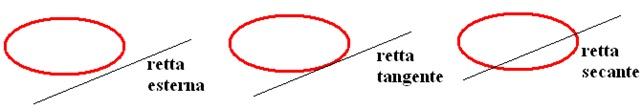
\includegraphics[width=\textwidth]{img/rettaconica.jpg}
  \caption{Posizioni reciproche tra una retta ed un'ellisse.}%
  %\label{fig:ellissedalcono}
  %    \end{inaccessibleblock}
\end{figure}
Geometricamente per stabilire la posizione di una retta rispetto ad una 
conica, disegniamo i due oggetti sul piano cartesiano e verifichiamo quanti 
punti hanno in comune. Algebricamente, per stabilire la posizione di una 
retta rispetto ad una conica andiamo a considerare il sistema delle due 
equazioni, quella della conica, ad esempio un'ellisse e quella della 
retta:
\[\begin{cases}  \dfrac{x^{2}}{a^{2}}+\dfrac{y^{2}}{b^{2}}=1   \\ y=mx+q  
\end{cases}\]
Il sistema si sviluppa in un'equazione di secondo grado nella quale il 
segno del $\Delta$ determina, la posizione reciproca fra retta ed ellisse:

\begin{itemize} [noitemsep]
  \item se $\Delta$<0, l'equazione di secondo grado non ha soluzioni 
reali e dunque retta e conica non hanno punti in comune, non si intersecano;
  \item se $\Delta$=0, l'equazione di secondo grado, deducibile dal 
sistema, ha due soluzioni coincidenti e quindi conica e retta hanno un solo 
punto in comune: la retta è tangente alla conica;
  \item se $\Delta$>0, l'equazione di secondo grado ha due soluzioni 
e di conseguenza i punti in comune tra retta e conica sono due: la retta è 
secante alla conica.
\end{itemize}

In generale per determinare le intersezioni tra una retta e una conica, 
trovando così la posizione relativa della retta rispetto alla conica, 
dobbiamo risolvere un sistema a due equazioni, quella della conica e quella 
della retta. 

Per fare una ulteriore applicazione studiamo le intersezioni tra una 
parabola e una retta.
Data la parabola di equazione P: y=a$ x^{2}+bx+c$ e la retta generica $r$: 
y=mx+q le loro intersezioni sono determinate dal sistema:
\[\begin{cases}  y=a x^{2} +bx+c   \\ y=mx+q  
\end{cases}\]
dal quale otteniamo l'equazione:
$ax^{2} +(b-m)x+c-q=0$
equazione di secondo grado in x, le cui soluzioni sono le ascisse dei punti 
di intersezione, a seconda del segno del $ \Delta $ dell'equazione ci 
saranno due soluzioni nel caso di retta secante, una nel caso di retta 
tangente e nessuna nel caso di retta esterna, come mostrato nela seguente 
figura:
\begin{figure}[htbp]
  \centering
  %    \begin{inaccessibleblock}[Cono a due falde tagliato da un piano
  %      che forma un'ellisse.]
  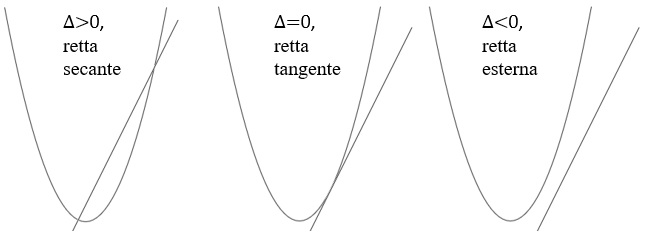
\includegraphics[scale=0.6]{img/rettaconica3.jpg}
  \caption{Posizioni reciproche tra una retta ed una parabola.}%
  %\label{fig:ellissedalcono}
  %    \end{inaccessibleblock}
\end{figure}

\begin{esempio} Data l'ellisse $ \dfrac{x^{2}}{16}+  
\dfrac{y^{2}}{4} =1$ e la retta $y=x+4$, stabilire la posizione della retta 
rispetto all'ellisse e le coordinate degli eventuali punti di intersezione. 
Secondo quanto visto il sistema da risolvere è:

$\begin{cases}  \dfrac{x^{2}}{16}+\dfrac{y^{2}}{4}=1   \\ y=x+4  
\end{cases}$  
sostituendo otteniamo l'equazione: $ 
\dfrac{x^{2}}{16}+\dfrac{x^{2}+8x+16}{4}=1$ che semplificata risulta: $5 
x^{2} +32x+48=0$.
con $ \Delta =64>0$. 

\begin{minipage}{.65\textwidth}
  La retta è dunque secante, calcoliamo ora i due punti di 
intersezione. 
  Risolvendo l'equazione otteniamo le ascisse dei punti di 
intersezione $ x_{1} =- \dfrac{12}{5} $ e $ x_{2} =-4$. Sostituendo tali 
ascisse nell'equazione della retta otteniamo le corrispondenti ordinate $ 
y_{1} =\dfrac{8}{5}$ e $ y_{2} =0$. I punti cercati sono $ P_{1}  
\left(-\dfrac{12}{5};~ \dfrac{8}{5}\right) $ e $ P_{2} =(-4;~0)$.
\end{minipage}
\hspace{.2cm}
\begin{minipage}{.3\textwidth}
  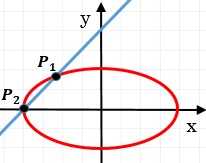
\includegraphics[width=\textwidth]{img/esempioposizione1.jpg}
  %    \caption{Generazione di un cono a due falde}% 
\end{minipage}
\end{esempio}
 
\section{Rette tangenti ad una conica}
\label{sec:coniche_tangenti}

Analizziamo ora, nello specifico, il caso di tangenza. In generale, per un 
punto esterno ad una conica possono esser condotte due tangenti mentre per 
un punto appartenente alla conica può essere condotta una sola tangente;  
da un punto interno alla conica, cioè dalla sua parte convessa, non si 
possono tracciare tangenti, come illustrato di seguito nel caso della 
parabola. 

\begin{figure}[t]
  \centering
  %    \begin{inaccessibleblock}[Cono a due falde tagliato da un piano
  %      che forma un'ellisse.]
  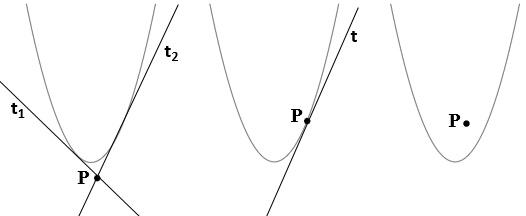
\includegraphics[scale=0.8]{img/tangenti2.jpg}
  \caption{Rette tangenti alla parabola.}%
  %\label{fig:ellissedalcono}
  %    \end{inaccessibleblock}
\end{figure}

Quanto appena visto per la parabola vale anche per le altre coniche.
Vogliamo ora determinare le rette tangenti ad una conica passanti per un 
punto dato. I casi possibili, come abbiamo appena visto, sono due: se il 
punto è esterno alla conica, in generale, si trovano due rette tangenti, se 
il punto appartiene alla conica, una sola tangente.

\subsection{Tangenti per un punto esterno ad una conica}

Per un punto esterno ad una conica passano due rette tangenti alla conica 
stessa. Per determinare le equazioni di queste tangenti, conoscendo la 
conica e le coordinate del punto esterno, in generale, si procede con il 
metodo del $ \Delta $=0. Andiamo ad illustrare per punti tale metodo:

\begin{itemize} [noitemsep]
  \item si scrive l'equazione del fascio di rette proprio centrato 
nel punto dato, avente m variabile: $y- y_{0} =m\left(x-x_{0}\right)$;
  \item si mette a sistema tale equazione con quella della conica 
data;
  \item si risolve il sistema per una variabile, x o y, trovando una 
equazione di secondo grado ad un parametro (m) e si determina il $ \Delta $ 
di tale equazione;
  \item ponendo $ \Delta $=0 si determinano i valori del parametro m 
che costituiscono i coefficienti angolari delle rette tangenti cercate, che 
si determinano sostituendo tali m trovati nell'equazione del fascio di 
rette iniziale.
\end{itemize}

  Poniamo attenzione a quest'ultimo punto, infatti, se l'equazione 
del $ \Delta $ è di secondo grado in m, i due m rappresentano i due 
coefficienti angolari delle due rette, se l'equazione del $ \Delta $ è di 
primo grado la sua soluzione rappresenterà il coefficiente di una retta 
tangente mentre l'altra tangente sarà fornita dalla retta verticale $x= 
x_{0} $. 

  Nella formula del fascio di rette infatti non è mai compresa la 
retta verticale passante per il centro del fascio, tale retta, per 
completare il fascio, va aggiunta alla formula del fascio:
  $y-y_{0} =m(x- x_{0} ) \cup x= x_{0} $
  

\begin{esempio} Determinare le equazioni delle tangenti 
all'ellisse $ x^{2} + \dfrac{y^{2}}{3} $=1 condotte dal punto $P(2;~0)$.

Procediamo come appena indicato. L'equazione del fascio di rette di centro 
P è $y-0=m(x-2)~ U ~x=2$, il sistema che otteniamo, mettendo insieme conica 
data e fascio appena determinato, è:
\[\begin{cases}  x^{2}+\dfrac{y^{2}}{3}=1   \\ y=mx-2m  
\end{cases} \sRarrow  
\begin{cases}  3x^{2}+y^{2}=3   \\ y=mx-2m  
\end{cases} \sRarrow  
\begin{cases}  3x^{2}+m^{2}x^{2}+4m^{2}-4m^{2}x-3=0   \\ y=mx-2m  
\end{cases}\]
riscriviamo l'equazione di secondo grado ottenuta, trovandone il $\Delta$ 
con la formula ridotta: \((3+ m^{2} ) x^{2} -4 m^{2} x+4 m^{2} -3=0\), 
\(\Delta =4 m^{4} -(3+ m^{2} )(4m^{2}-3)=
4 m^{4} -12 m^{2} +9-4 m^{4} +3 m^{2} =-9 m^{2} +9\). 
Ponendo il $\Delta$=0 e risolvendo 
l'equazione pura che si trova abbiamo \(m_{1} = 1\) e \(m_{2} = -1\).

Sostituiamo gli m appena trovati nell'equazione del fascio per trovare le 
rette tangenti: \(y=x-2\) e \(y=-x+2\).
\end{esempio}

\begin{esempio} Determinare le equazioni delle tangenti 
all'ellisse \(x^{2} + \dfrac{y^{2}}{3} =1\) condotte dal punto 
\(P\punto{1}{2}\).

L'equazione del fascio di rette di centro \(P\) è \(y-2=m(x-1) U x=1\), il 
sistema che otteniamo, mettendo insieme conica data e fascio appena determinato 
è:
\[\begin{cases}  x^{2}+\dfrac{y^{2}}{3}=1   \\ y=mx-m+2  
\end{cases} \sRarrow  
\begin{cases}  3x^{2}+y^{2}=3   \\ y=mx-m+2  
\end{cases} \sRarrow 
\begin{cases}  3x^{2}+m^{2}x^{2}+m^{2}+4-2m^{2}x-4m+4mx-3=0   \\ y=mx-m+2  
\end{cases}\]
l'equazione di secondo grado risulta: 
$\left(3+ m^{2} \right) x^{2} +2\left(2m-m^{2} \right)x+ m^{2} -4m+1=0$ 
e il $\Delta$ della formula 
ridotta è 
$\Delta =4 m^{2} + m^{4} -4 m^{3} -\tonda{3+ m^{2}}\tonda{m^{2}-4m+1}=
4 m^{2} + m^{4} -4 m^{3} -3 m^{2} +12m-3- m^{4} +4 m^{3} - m^{2} =12m-3$. 
Ponendo ora $\Delta =0$, otteniamo che $m=\dfrac{1}{4}$. 
Essendo il $\Delta$ di primo grado il possibile m, coefficiente angolare, 
è soltanto uno e la corrispondente retta risulta 
$y-2=\dfrac{1}{4}(x-1) \longrightarrow  4y-x-7=0$. 
L'altra retta tangente è la retta verticale passante per il punto P: \(x=1\).
\end{esempio}

\subsection{Tangente per un punto appartenente alla conica}

Se il punto, per il quale si vogliono cercare le tangenti ad una conica, 
appartiene alla conica, necessariamente si troverà una sola retta tangente. 
Per trovare tale retta si può ricorrere ancora al metodo precedente del 
sistema tra conica e fascio di rette, ponendo poi il $ \Delta $=0, ma si 
preferisce, in questo caso, usare il meno complesso metodo dello 
sdoppiamento. Tale metodo evita di impostare e risolvere il sistema a due 
equazioni di secondo grado e con una semplice sostituzione si trova 
immediatamente la retta tangente cercata.
Andiamo ad illustrare per punti tale metodo, utilizzando come esempio di 
conica una circonferenza, ma sottolineando subito che tale metodo può 
essere applicato ad una qualsiasi conica:

\begin{itemize} [noitemsep]
  \item   dato il punto $P( x_{0};~ y_{0} )$ appartenente alla 
circonferenza e scritta l'equazione canonica della circonferenza $ x^{2} + 
y^{2} +ax+by+c=0$ si procede con la seguente sostituzione:

$ x^{2} \longrightarrow x x_{0} $;~$ y^{2} \longrightarrow y y_{0}$;~
$x= \dfrac{x+x_{0}}{2} $;~$y= \dfrac{y+y_{0}}{2}$

  \item otteniamo la seguente equazione che rappresenta la retta 
tangente cercata:

  $x x_{0} +y y_{0}+a \dfrac{x+x_{0}}{2}  +b \dfrac{y+y_{0}}{2} +c=0$
\end{itemize}

\begin{esempio} Determinare l' equazione della tangente 
all'ellisse $ \dfrac{x^{2}}{25}+\dfrac{y^{2}}{36} =1$ passante per il suo 
punto $P\left(3;~-\dfrac{24}{5}\right)$. 
Procediamo come appena indicato, mediante il metodo dello sdoppiamento. 
Applichiamo le sostituzioni appena viste:
\[\dfrac{xx_{0}}{25} + \dfrac{yy_{0}}{36} = 1  \longrightarrow 
\dfrac{3x}{25} - \dfrac{24y}{5 \cdot 36} =1  \longrightarrow  
\dfrac{108x-120y}{900}=\dfrac{900}{900} \longrightarrow 9x-10y-75=0\]
\end{esempio}

\section{Curve deducibili dalle equazioni delle coniche}
\label{sec:coniche_curve_deducibili}

La conoscenza delle equazioni e delle proprietà delle coniche consente di 
rappresentare graficamente alcune tipologie di funzioni irrazionali.\\ 
Vediamone un esempio: tracciamo il grafico della funzione 
$y=\sqrt{4-9x^{2}}$. Innanzitutto la funzione è definita solo se il 
radicando è non negativo, cioè se $4-9x^{2}\geq0$ e questa disequazione è 
risolta per $ -\dfrac{2}{3}\leq x\leq \dfrac{2}{3}$. il secondo membro 
dell'equazione risulta così non negativo e per mantenere l'uguaglianza 
anche il primo membro deve essere non negativo, otteniamo dunque $ y\geq0 $. 
Ora con le condizioni poste possiamo elevare al quadrato entrambi i membri 
per eliminare la radice, ottenendo $ y^{2}=4-9x^{2} $ che non è altro che 
l'equazione di un'ellisse: $ 9x^{2}+y^{2}=4 $.

Quanto appena visto equivale all'impostazione del sistema:

\[\begin{cases}  4-9x^{2}\geq0   \\ y\geq0  \\y^{2}=4-9x^{2} 
\end{cases} \sRarrow
\begin{cases}   -\dfrac{2}{3}\leq x\leq \dfrac{2}{3}   \\ y\geq0  \\ 
y=\sqrt{4-9x^{2}} \end{cases}\] 

% \begin{figure} [h]
\noindent \begin{minipage}{.75\textwidth}
La soluzione grafica di questo sistema è un'ellisse che ha 
dei limiti sia in ascissa che in ordinata, per tener conto di $ y\geq0 $ 
dobbiamo prendere solo la parte dell'ellisse con orinata positiva o nulla, 
cioè la parte di ellisse contenuta nel primo e secondo quadrante; e tenendo 
conto dei limiti sulle ascisse si ottiene il grafico a fianco.
  \end{minipage}
  \hfill
  \begin{minipage}{.2\textwidth}
    %    \begin{inaccessibleblock}[Cono a due falde tagliato da un piano
    %      che forma un'ellisse.]
    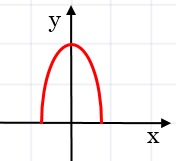
\includegraphics[width=\textwidth]{img/curva1.jpg}
%     \caption{Grafico dell'equazione $ y=\sqrt{4-9x^{2}} $.}
    %\label{fig:ellissedalcono}
    %    \end{inaccessibleblock} 
  \end{minipage}
% \end{figure}

Consideriamo un altro esempio: $y=2-\sqrt{6x-x^{2}}  $ e proviamo a 
disegnarne il grafico corrispondente. Come primo passo riscriviamo la 
funzione come $y-2=-\sqrt{6x-x^{2}}  $, poi cerchiamo di impostare un 
sistema simile al precedente che rispetti le condizioni di esistenza del 
radicale e le sue conseguenze:
\[\begin{cases}  6x-x^{2}\geq0   \\ y-2\leq0  \\y^{2}-4y+4=6x-x^{2} 
\end{cases} \sRarrow
\begin{cases}   0\leq x\leq6   \\ y\leq2  \\ x^{2}+y^{2}-6x-4y+4=0 
\end{cases}\]
L'ultima equazione diventa:
\[y^{2}-4y+4=x^{2}+6x \sRarrow \tonda{y-2}^2 = - x^{2}+6x \sRarrow
y-2 = \sqrt{- x^{2}+6x} \sRarrow y=2-\sqrt{-x^{2} +6x}\]

% \begin{figure} [h]
\noindent \begin{minipage}{.75\textwidth}
La prima disequazione rappresenta di nuovo le condizioni del 
radicale, la seconda disequazione ci ricorda che il primo membro, \(y-2\), deve 
avere lo stesso segno del secondo, che essendo una radice con il segno 
negativo davanti, non può essere positivo, infine l'equazione rappresenta 
una circonferenza di 
centro \(\punto{3}{2}\) e raggio~3. Il grafico cercato è dunque quello di una 
circonferenza con le caratteristiche trovate limitata nelle ordinate a 
$y\leq2$ e nelle ascisse a $ 0\leq x\leq6 $.
  \end{minipage}
  \hfill
  \begin{minipage}{.2\textwidth}
    %    \begin{inaccessibleblock}[Cono a due falde tagliato da un piano
    %      che forma un'ellisse.]
    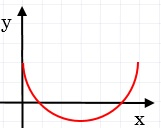
\includegraphics[width=\textwidth]{img/curva2.jpg}
%     \caption{Grafico dell'equazione $ y=2-\sqrt{6x-x^{2}} $.}
    %\label{fig:ellissedalcono}
    %    \end{inaccessibleblock} 
  \end{minipage}
% \end{figure}

% \begin{figure} [h]
\noindent 
\begin{minipage}{.2\textwidth}
  %    \begin{inaccessibleblock}[Cono a due falde tagliato da un piano
  %      che forma un'ellisse.]
  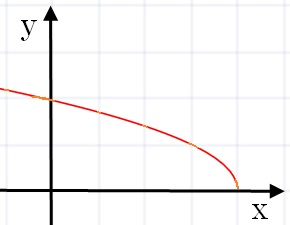
\includegraphics[width=\textwidth]{img/curva3.jpg}
%   \caption{Grafico dell'equazione $ y=\sqrt{4-x} $.}
  %\label{fig:ellissedalcono}
  %    \end{inaccessibleblock} 
\end{minipage}
  \hfill
\begin{minipage}{.75\textwidth}
Ancora un esempio che riguarderà stavolta la parabola. 
Vogliamo disegnare il grafico di $ y=\sqrt{4-x} $, il sistema 
corrispondente è:
\[\begin{cases}  4-x\geq0   \\ y\geq0  \\y^{2}=4-x 
\end{cases} \sRarrow
\begin{cases}   x\leq4   \\ y\geq0  \\ x=-y^{2}+4 
\end{cases}\]
otteniamo una parabola con l'asse parallelo all'asse Y e di questa parabola 
prendiamo in considerazione solo la parte con y non negativa.
  \end{minipage}
% \end{figure}


